\documentclass{article}

\usepackage{fancyhdr}
\usepackage{extramarks}
\usepackage{xcolor}
\usepackage{amsmath}
\usepackage{amsthm}
\usepackage{amssymb}
\usepackage{amsfonts}
\usepackage{tikz}
\usepackage[plain]{algorithm}
\usepackage{algpseudocode}
\usepackage[left=1in]{geometry}
\usepackage[shortlabels]{enumitem}
\usepackage{transparent}
\usetikzlibrary{automata,positioning}


%%%%%%%%%%%%%%%%%%%%%%%%%%%%%%%%%%%%%%%%%%%%%%%%%%%%%%%%%%%%%%%%%%%%%%%%%
%%%%%%%%%%%%%%%%%%%%%%%%%%%%% PDF COLOR %%%%%%%%%%%%%%%%%%%%%%%%%%%%%%%%%
%%%%%%%%%%%%%%%%%%%%%%%%%%%%%%%%%%%%%%%%%%%%%%%%%%%%%%%%%%%%%%%%%%%%%%%%%
\usepackage{xcolor} \pagecolor[rgb]{0,0,0} \color[rgb]{0.9,0.9,0.9}
%%%%%%%%%%%%%%%%%%%%%%%%% SUPPRESS UNDERFULL HBOX %%%%%%%%%%%%%%%%%%%%%%%
\hbadness = 20000
%%%%%%%%%%%%%%%%%%%%%%%%%%%%%%%%%%%%%%%%%%%%%%%%%%%%%%%%%%%%%%%%%%%%%%%%%
%
% Basic Document Settings 
%
\topmargin=-0.75in
\evensidemargin=0in
\oddsidemargin=0in
\textwidth=6.5in
\textheight=9.0in
\headsep=0.25in

\linespread{1.1}
\fancypagestyle{plain}{}
\pagestyle{fancy}
\fancyhf{}

\chead{\hmwkClass: \hmwkTitle}
\lfoot{\lastxmark}
\cfoot{\thepage}

\renewcommand\headrulewidth{0.4pt}
\renewcommand\footrulewidth{0.4pt}

\setlength\parindent{0pt}

\newcommand{\bd}{\textbf}
\newcommand{\hmwkTitle}{Homework\ \#2}
\newcommand{\hmwkClass}{Computational Modules}

\newcommand{\nat}{\mathbb{N}}
\newcommand{\lang}{\mathcal{L}}
\newcommand{\AB}{\Sigma}
\newcommand{\ch}{\sigma}
\newcommand{\de}{\delta}
\newcommand{\empw}{\varepsilon}
\newcommand{\ceq}[1]{\overset{#1}{\thicksim}}
\newcommand{\nceq}[1]{\overset{#1}{\nsim}}



% use for comment block, surround block with "\/*" and at the end "*/" 
\long\def\/*#1*/{}


%%%%%%%%%%%%%%%%%%%%%%%%%%%%%%%%%%%%%%%%%%%%%%%%%%%%%%%%%%%%%%%%%%%%%%%%%

\newcommand{\hmwkAuthorName}{\bd{Michael Zhitomirsky}, ID 321962714}

%%%%%%%%%%%%%%%%%%%%%%%%%%%%%%%%%%%%%%%%%%%%%%%%%%%%%%%%%%%%%%%%%%%%%%%%%

%
% Title 
%

\title{
    \textmd{\bd{\hmwkClass:\ \hmwkTitle}}\\
}
\author{\hmwkAuthorName}

\begin{document}

\maketitle
\thispagestyle{firststyle}

\begin{enumerate}
      \item Prove:
            \begin{enumerate}
                  \item 
$\lang''=\{x_1 x_2 . . . x_k : k \in \nat ,x_i \in \AB \text{ for every }
    1 \leq i \leq k \\ \text{ and } \exists y_1,y_2,...y_{2k} \in \AB
    \text { such that } x_1 y_1 y_2 x_2 y_3 y_4...x_k y_{2k-1} y_{2k} \in \lang \}$
\\ \\
We shall construct the following NFA $N''$ for $\lang''$: \\
$N''=(Q, \AB, \de'', S=\{q_0\}, F)$, such that the
transition function is: \\
$\de''(q,\ch)=\{\de(\de(\de(q,\ch),a),b) : \forall a,b \in \AB\},
    \forall q \in Q, \forall \ch \in \AB$. \\
Meaning that $\de''$ is using $\de$ to make one step with $\ch$ and
then 'guess' two steps with all possible symbols in $\AB$.
\\ \\
Now, we shall prove its correctness: \\
We need to show that: $w \in \lang'' \Longleftrightarrow  w \in \lang(N'')$. \\
Note that: \\
$w \in \lang''$\\

(From definition of $\lang''$) \\
$\Longleftrightarrow w \in \{x_1 x_2 . . . x_k : k \in \nat ,x_i \in \AB \text{ for every }
    1 \leq i \leq k \\ \text{ and } \exists y_1,y_2,...y_{2k} \in \AB
    \text { such that } x_1 y_1 y_2 x_2 y_3 y_4...x_k y_{2k-1} y_{2k} \in \lang \}$  \\

(From definition of $A$: $\lang = \lang(A)$) \\
$\Longleftrightarrow \exists k \in \nat ,x_1...x_k \in \AB^*:  w=x_1 x_2 . . . x_k, \\
    \text{ and } \exists y_1,y_2,...y_{2k} \in \AB
    \text { such that } w_{\lang}=x_1 y_1 y_2 x_2 y_3 y_4...x_k y_{2k-1} y_{2k} \in \lang=\lang(A)$ \\

(From definition of $A$) \\
$\Longleftrightarrow \exists q_1,q_2,...q_{3k} \text{ s.t. } $\\
$
    \de(q_0,x_1)=q_1, \de(q_1,y_1)=q_2, \de(q_2,y_2)=q_3, ..., \\
    \de(q_{3k-3},x_{k})=q_{3k-2}, \de(q_{3k-2},y_{2k-1})=q_{3k-1}, \de(q_{3k-1},y_{2k})=q_{3k} \in F
$ \\ \\
(*) Now, from the above and the definition of $\de''$ we get that: \\
$\exists q_1,q_2,...q_{3k} \text{ s.t. } $\\
$
    \de''(q_0,x_1)=\{\de(\de(\de(q_0,x_1),a),b) : \forall a,b \in \AB\} \ni q_3 \text{ } (q_0 \in S), ..., \\
    \de''(q_{3i-3},x_{i})=\{\de(\de(\de(q_{3i-3},x_{i}),a),b) : \forall a,b \in \AB\} \ni q_{3i}, ..., \\
    \de''(q_{3k-3},x_{k})=\{\de(\de(\de(q_{3k-3},x_{k}),a),b) : \forall a,b \in \AB\} \ni q_{3k} \text{ } (q_{3k} \in F)
$ \\ \\

(From definition of $N''$) \\
$\Longleftrightarrow w=x_1 x_2 . . . x_k \in \lang(N'')$ \\
\\
Note that when looking at the proof in the direction of - ($w \in \lang'' \Longleftarrow  w \in \lang(N'')$),
we get transition (*) by choosing  $y_1,y_2,...y_{2k}$ from the specific $a,b \in \AB$ that give us the
accepting branch in the NFA $N''$ for input $w=x_1 x_2 ... x_k$.
\\

In conclusion, we got $w \in \lang'' \Longleftrightarrow  w \in \lang(N'')$. Thus, concluding the proof. \\


                        \pagebreak
                  \item $\lang''=\{xy : yx \in \lang \}$
\\ \\
The idea would be to construct an NFA per state $q \in Q$, $N_q$,
each NFA will check if we can 'break' the word $yx \in \lang$ in state q of $A$.
So each NFA will contain 2 copies of $A - A_{q,1}, A_{q,2}$ such that for
$yx \in \lang$, $x$ will take us from state q in $A_{q,1}$ to $F_{q,1}$
which will be connected with $\empw$-moves to $q_{0,q,2}$ in $A_{q,2}$,
and y will take us from there to state q in $A_{q,2}$.

The main NFA, $N''$, will be a 'union' of the he smaller NFAs ($N_q, \forall q \in Q$).
It will have an initial state group that is the group of the initial states of each of the
smaller NFAs ($N_q, \forall q \in Q$), and that way we will check if word $w$
is some rotation of some word in $\lang$.

Now, we shall give formal definitions for every one of the NFAs: \\

\underline{$\forall q \in Q, N_q$:} \\

$N_q=(Q \times \{1,2\} \times \{q\}, \AB, \de_q, S_q=\{(q, 1, q)\}, F_q=\{(q, 2, q)\})$, \\
such that the transition function is: \\
\[
    \de_q((q', k, q),\ch) = \left.
    \begin{cases}
        \{(\de(q',\ch)\}, k, q)\} , & \ch \in \AB                          \\
        \{(q_0, 2, q)\},            & q' \in F \wedge k=1 \wedge \ch=\empw \\
    \end{cases}
    \right\} , \text{ } k \in \{1,2\}, \ch \in \AB \cup \{\empw\}
\]

\underline{$N''$:} \\

$N''=((Q \times \{1,2\} \times Q), \AB, \de'',
    S''=\{(q_i, 1, q_i) : q_i \in Q\}, F''=\{(q_f, 2, q_f) : q_f \in Q\})$, \\
such that the transition function is: \\
\[
    \de''((q', k, q),\ch) = \de_{q}((q', k, q),\ch),  k \in \{1,2\}, \ch \in \AB \cup \{\empw\}
\]

Now, we shall prove its correctness: \\
We need to show that: $w \in \lang'' \Longleftrightarrow  w \in \lang(N'')$. \\
Note that: \\
$w \in \lang''$\\

(From definition of $\lang''$) \\
$\Longleftrightarrow w \in \{xy : yx \in \lang \}$ \\

(From definition of $A$: $\lang = \lang(A)$) \\
$\Longleftrightarrow \exists x=x_1...x_n,y=y_1...y_m \in \AB^* : w=xy \wedge yx \in \lang = \lang(A)$ \\
\\ \\

(From definition of $A$) \\
$\Longleftrightarrow \exists q_1,q_2,...q_m, q_{m+1}...q_{n+m} \text{ s.t. } $\\
$
    \de(q_0,y_1)=q_1, \de(q_1,y_2)=q_2, ..., \\
    \de(q_{m-1},y_m)=q_m, \de(q_m,x_1)=q_{m+1},...,\\
    \de(q_{n+m-1},x_{n})=q_{n+m} \in F
$ \\

(From definition of $\de''$) \\
$\Longleftrightarrow \exists q_1,q_2,...q_m, q_{m+1}...q_{n+m} \text{ s.t. } $\\
$
    \de''((q_m, 1, q_m), x_1) \ni (q_{m+1}, 1, q_m) \text{ } ((q_m, 1, q_m) \in S''), ..., \\
    \de''((q_{n+m-1}, 1, q_m), x_n) \ni (q_{n+m}, 1, q_m),\\
    \de''((q_{n+m}, 1, q_m), \empw) \ni (q_0, 2, q_m), (q_{n+m} \in F)\\
    \de''((q_0, 2, q_m), y_1) \ni (q_1, 2, q_m), ...,\\
    \de''((q_{m-1}, 2, q_m), y_m) \ni (q_m, 2, q_m) \text{ } ((q_m, 2, q_m) \in F'')
$ \\

(From definition of $N''$) \\
$\Longleftrightarrow w=x_1...x_n y_1... y_m \in \lang(N'')$ \\

All in all, we got $w \in \lang'' \Longleftrightarrow  w \in \lang(N'')$. Thus, concluding the proof. \\

            \end{enumerate}

            \pagebreak

      \item Formally describe a 2-tape non-deterministic TM that on input $\#1^n\#$ such
that $n > 1$ chooses non-deterministically $i, j$ such that $0 < i, j \leq n$, writes
$1^i\#1^j$ on the second tape and accepts. You may use a model that allows the
head to stay put (S) as well as moving right (R) and left (L). \\

We will denote the required TM by $M$. \\
The formal description of $M$ will be: \\
$ M = (Q, \AB, \Gamma, \de, q_0, q_a, q_r) $ such that: \\
$ Q      = \{q_0, q_i, q_j, q_a, q_r\} $ \\
$ \AB    = \{1, \#\} $ \\
$ \Gamma = \AB \cup \{\sqcup\} $ \\
and $\de$ is defined by:

\begin{figure}[h]
    \centering
    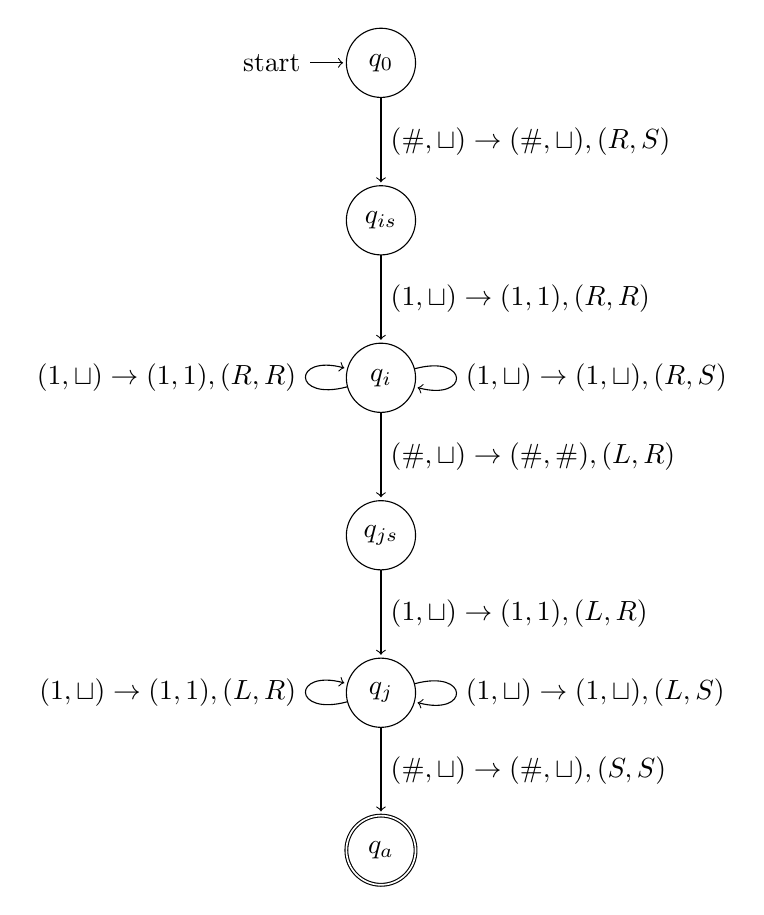
\begin{tikzpicture}[shorten >=1pt,node distance=2cm,on grid,auto]
        \node[state, initial]   (q_0)                  {$q_0$};
        \node[state]            (q_is) [below=of q_0]  {$q_{is}$};
        \node[state]            (q_i)  [below=of q_is] {$q_i$};
        \node[state]            (q_js) [below=of q_i]  {$q_{js}$};
        \node[state]            (q_j)  [below=of q_js] {$q_j$};
        \node[state, accepting] (q_a)  [below=of q_j]  {$q_a$};

        \path[->]
        (q_0)
        edge              node {$(\#, \sqcup) \rightarrow (\#,\sqcup), (R,S)$} (q_is)

        (q_is)
        edge              node {$(1, \sqcup)  \rightarrow (1,1),       (R,R)$} (q_i)

        (q_i)
        edge [loop left]  node {$(1, \sqcup)  \rightarrow (1,1),       (R,R)$} (q_i)
        edge [loop right] node {$(1, \sqcup)  \rightarrow (1, \sqcup), (R,S)$} (q_i)
        edge              node {$(\#, \sqcup) \rightarrow (\#,\#),     (L,R)$} (q_js)

        (q_js)
        edge              node {$(1, \sqcup)  \rightarrow (1,1),       (L,R)$} (q_j)

        (q_j)
        edge [loop left]  node {$(1, \sqcup)  \rightarrow (1,1),       (L,R)$} (q_j)
        edge [loop right] node {$(1, \sqcup)  \rightarrow (1, \sqcup), (L,S)$} (q_j)
        edge              node {$(\#, \sqcup) \rightarrow (\#,\sqcup), (S,S)$} (q_a);

    \end{tikzpicture}
    \label{fig:multiple5}
\end{figure}


Short explanation: \\
1. First we go over the input from left to right and each time we see '1' we choose
to write '1' on the second tape or write nothing and move on.

2. When we reach the end of the input we have written the '$1^i$' part on the second tape, so we write '$\#$'.

3. Then we go over the input from right to left and repeat the process - each time we
see '1' we choose to write '1' on the second tape or write nothing and move on.

4. When we reach the beginning of the tape, at that point we have written '$1^i\#1^j$' on the second tape,
where $i, j$ were chosen non-deterministically.


            \pagebreak

      \item Let us define a function $f$ to be {\it shrinking} if there exists $n_0 \in \nat$ such that
            for every $x \in \AB^*$ it holds that if $n_0 \leq |x|$ then $|f(x)| < |x|$.
            Assuming $\Pcl \neq \NPcl$, prove/disprove:

            \begin{enumerate}
                  \item If $\lang_1, \lang_2 \in \Pcl$ are non-trivial ($\lang_1, \lang_2 \notin \{\emptyset, \AB^*\}$), then there exists a polynomial shrinking
reduction from $\lang_1$ to $\lang_2$.
                  \item If $\lang_1, \lang_2 \in \NPcl$ are non-trivial ($\lang_1, \lang_2 \notin \{\emptyset, \AB^*\}$), then there exists a polynomial shrinking
reduction from $\lang_1$ to $\lang_2$.


if there is reduction then whole NP is NPC, beacuse P is NP we get P in NPC, then P=NP=NPC
                        \pagebreak
                  \item $\lang=\{w : \exists n \in \nat \text{ s.t. } |w| = n^3\}$
(twice, once using the pumping lemma and once using Myhill-Nerode)

\underline{Using Pumping Lemma} \\

We will prove by contradiction - we will assume that $\lang$ is regular.
Since $\lang$ is regular, we can apply the pumping lemma to $\lang$. Let $k$
be the number from the pumping lemma for $\lang$. We will choose $w = 0^{3^k}$.
Note that $|w|=3^k \rightarrow w \in \lang \text{ and } |w| \geq k$.
Therefore, from the pumping lemma, there exists some $x, y, z$ where $w = xyz$ and:

\begin{enumerate}
    \item $\forall i \geq 0: x y^i z \in \lang$
    \item $|y| > 0$
    \item $|xy| \leq k$
\end{enumerate}

From (ii) and (iii) we get that $y=0^j, 0 < j \leq k$,
note that $x y^2 z = 0^{k^3} 0^j = 0^{k^3+j}$,
so we get
\[
    |x y^2 z| = k^3+j
\]
but
\[
    k = \sqrt[3]{k^3} < \boldsymbol{\sqrt[3]{k^3+j}} < \sqrt[3]{k^3+k} < \sqrt[3]{k^3+3k^2+3k+1} = \sqrt[3]{(k+1)^3} = k+1
\]
so $\sqrt[3]{k^3+j} \notin \nat$, meaning $x y^2 z \notin \lang$ in contradiction with (i). \\
We got a contradiction, hence $\lang$ is not regular. \\


\underline{Using Myhill-Nerode Theorem} \\

Note that for $i < j$ we get $x = 0^{i^3+1} \nceq{\lang} 0^{j^3+1}  = y$,
since for $z=0^{3i^2+3i} \in \AB^*$ we get:

$xz = 0^{i^3+1}0^{3i^2+3i}=0^{i^3+3i^2+3i+1}=0^{(i+1)^3} \in \lang \text{ } (\sqrt[3]{|xz|}=\sqrt[3]{(i+1)^3}=i+1 \in \nat$, \\
but $yz = 0^{j^3+1}0^{3i^2+3i}=0^{j^3+3i^2+3i+1}$, so:
\[
    |yz| = j^3+3i^2+3i+1
\]
and
\[
    j = \sqrt[3]{j^3} < \boldsymbol{\sqrt[3]{j^3+3i^2+3i+1}} < \sqrt[3]{j^3+3j^2+3j+1} = \sqrt[3]{(j+1)^3} = j+1
\]
so $\sqrt[3]{j^3+3i^2+3i+1} \notin \nat$, meaning $yz \notin \lang$.

Hence, each $ 0^{i^3+1} $ belongs to a different equivalence class for every $i \geq 0$, \\
meaning $|\AB^* / \ceq{\lang}| \geq |\{0^{i^3+1}: i \geq 0\}| = \infty$ \\
We got that $\lang$ has an infinite number of equivalence classes, hence from
Myhill-Nerode Theorem we get that $\lang$ is not regular. \\
            \end{enumerate}


      \item
            \begin{enumerate}
                  \item polynomial verifier runtime is at most $p(|x|)$, hence it would not look beyond the first $p(|x|)$ symbols of $w$,
hence $w$ can be of length at most $p(|x|)$.
If the length of $w$ is less than $p(|x|)$, then we can pad $w$ until its length reaches exactly $p(|x|)$
In conlusion there is a verifier for $\lang$ that only accepts cerificates of length exactly $p(|x|)$
(its behaviour would be identical to the behaviour of the standard verifier with the addional check
that the length of the cerificate it receives as input is exactly $p(|x|)$, if it is not - it rejects.)

***build the verfier***
                  \item Prove that $CIRSAT \in \NPCcl$ (use ”the heart of Cook-Levin” from Lecture 10).  \\

Proof: \\
We need to show that: \\
1. $CIRSAT \in NP$ \\
2. $\forall \lang \in \NPcl: \lang \leq_p CIRSAT$ \\

First we show that $CIRSAT \in NP$, by building a polynomial verifier $V$ for it. \\
$V$ for input $(\langle C, x \rangle, w)$:
\begin{enumerate}[1., itemsep=5pt]
    \item Verify that $\langle C, x \rangle$ is a valid encoding of a boolean circuit and a partial input, if it's not - reject.

    \item Calculate $C(xw)$

    \item If $C(xw)=1$ - accept, otherwise - reject.

\end{enumerate}

Indeed: \\
If $\langle C, x \rangle \in CIRSAT$ \\
$\Rightarrow \langle C, x \rangle$ is a valid encoding of boolean circuit and a partial input
and there exists $w \in \AB^*$ such that $C(xw)=1$. \\
$\Rightarrow $ There exists $w \in \AB^*$ such that $V$ accepts $(\langle C, x \rangle, w)$. \\

If $\langle C, x \rangle \notin CIRSAT$ \\
$\Rightarrow \langle \phi \rangle$ is not a valid encoding of a boolean circuit and a partial input
or there doesn't exist $w \in \AB^*$ such that $C(xw)=1$. \\
If $\langle C, x \rangle$ is not a valid encoding of a boolean circuit and a partial input $\Rightarrow V$ rejects. \\
If there doesn't exist $w \in \AB^*$ such that $C(xw)=1$ \\
$\Rightarrow V$ rejects $(\langle C, x \rangle, w)$ for every $w \in \AB^*$.

Also $V$'s runtime on input $(\langle C, x \rangle, w)$ (where $|\langle C, x \rangle|=n$) is: \\
- For step (1): $O(q(n))$ for some polynomial function $q$ \\
- For step (2): $O(k(n))$ for some polynomial function $k$ \\
- For step (3): $O(1)$ \\
Thus, the total runtime of $V$ on input  $(\langle C, x \rangle, w)$ is polynomial in $|\langle C, x \rangle|=n$, so \underline{$CIRSAT \in \NPcl$}. \\

\pagebreak

Now we show that $\forall \lang \in \NPcl: \lang \leq_p CIRSAT$ \\
Let there be $\lang \in \NPcl$, therefore there exists a polynomial verifier $V_\lang$ for $\lang$, that only accepts
certificates of length exactly $p(|x|)$, where $p$ is the polynomial runtime of the verifier (we get this from the previuos section). \\

From ”the heart of Cook-Levin” in Lecture 10, for a TM $M$ that runs in time $t(n)$
there exists a function that is computable in time $g(t(n))$ (where $g$ is a polynomial function), that given $1^n$ as input, calculates
the encoding of a boolean circuit $C_{M,n}: \{0,1\}^n \rightarrow \{0,1\}$
such that: \\
1. $\forall z \in \{0,1\}^n: M(z)$ accepts $\iff C_{M,n}(z)=1$ \\
2. $|C_{M,n}| \leq O(t^2(n))$ \\

We denote the function that calculates the encoding of the boolean circuit in ”the heart of Cook-Levin” by $f$. \\
We will use the verifier $V_\lang$ as the TM in ”the heart of Cook-Levin”.

Now we will show that there is a polynomial reduction from $\lang$ to $CIRSAT$: \\
We define the following reduction $h: \AB^* \rightarrow \AB^*$:
$h(x) = (\langle f(1^{|x|+p(|x|)}), x \rangle)$

Notice that $h$ is computable in polynomial time, since it takes $O(g(p(n+p(n))))$ (where $|x|=n$ and $g$, $p$ are polynomial functions)
to calculate $f(1^{|x|+p(|x|)})$.

Also $\forall x \in \AB^*$:

If $x \in \lang$ \\
$\Rightarrow $ There exists $w \in \AB^{p(|x|)}$ such that $V_\lang$ accepts $(x, w)$. \\
$\Rightarrow $ From (1) of ”the heart of Cook-Levin”, for $h(x) = (\langle f(1^{|x|+p(|x|)}), x \rangle) = (\langle C, x \rangle)$,
we get $C(xw)=1$ \\
$\Rightarrow h(x) = (\langle f(1^{|x|+p(|x|)}), x \rangle) \in CIRSAT$ \\

If $x \notin \lang$ \\
$\Rightarrow V$ rejects $(x, w)$ for every $w \in \AB^*$. \\
$\Rightarrow $ From (1) of ”the heart of Cook-Levin”, for $h(x) = (\langle f(1^{|x|+p(|x|)}), x \rangle) = (\langle C, x \rangle)$,
we get $C(xw)=0$ for every $w \in \AB^{p(|x|)}$ \\
$\Rightarrow h(x) = (\langle f(1^{|x|+p(|x|)}), x \rangle) \notin CIRSAT$ \\

So we get \underline{$\lang \leq_p CIRSAT$}. \\
In conclusion, $CIRSAT \in \NPCcl$. As required.

            \end{enumerate}

            \pagebreak

      \item Prove that the following decision problems are in $\NPCcl$

            \begin{enumerate}
                  \item Input: sets $A_1, ..., A_n$, and a number $k$. \\
Question: do there exist $k$ mutually disjoint sets $A_{i_1} , ..., A_{i_l}$

We need to show that: \\
$\lang = \{\langle A = \{A_1, ..., A_n\}, k \rangle: \text{ there is a subset
        of A of k mutually disjoint sets}\} \in \NPCcl$ \\

Proof: \\
We will show that: \\
1. $\lang \in NP$ \\
2. $\forall \lang' \in \NPcl: \lang' \leq_p \lang$ by showing that $IS \leq_p \lang$ (we can do this since $IS \in NPC$) \\

First we show that $\lang \in NP$, by building a polynomial verifier $V$ for it. \\
$V$ for input $(\langle A = \{A_1, ..., A_n\}, k \rangle, w)$:
\begin{enumerate}[1., itemsep=5pt]
    \item Verify that $\langle A = \{A_1, ..., A_n\}, k \rangle$ is a valid encoding of a set of sets and a number, if it's not - reject.
    \item Verify that $w$ is a valid encoding of a subset of size $k$ in $A$ - $A_{i_1} , ..., A_{i_l}$, if it's not - reject.

    \item For every 2 sets in the subset - $A_j, A_l$
    \item \qquad If $A_j \cap A_l \neq \emptyset$ - reject. (Check this by comparing every element in $A_j$ with every element in $A_l$)

    \item Accept.

\end{enumerate}

Notice that steps (3-4) check whether the subset is indeed a mutually disjoint sets of size $k$.\\

So we get: \\
If $\langle A = \{A_1, ..., A_n\}, k \rangle \in \lang$ \\
$\Rightarrow \langle A = \{A_1, ..., A_n\}, k \rangle$ is a valid encoding of a set of sets and a number
and there is a subset of $A$ of size $k$ of mutually disjoint sets - $A_{i_1} , ..., A_{i_l}$.\\
$\Rightarrow $ For $w=\langle A_{i_1} , ..., A_{i_l} \rangle$, $V$ will verify that indeed every 2 sets in the
subset are mutually disjoint and accept. \\
$\Rightarrow $ There exists $w \in \AB^*$ such that $V$ accepts $(\langle A = \{A_1, ..., A_n\}, k \rangle, w)$. \\

If $\langle A = \{A_1, ..., A_n\}, k \rangle \notin \lang$ \\
$\Rightarrow \langle A = \{A_1, ..., A_n\}, k \rangle$ is not a valid encoding of a set of sets and a number
or there doesn't exist a subset of $A$ of size $k$ of mutually disjoint sets. \\
If $\langle A = \{A_1, ..., A_n\}, k \rangle$ is not a valid encoding of a set of sets and a number $\Rightarrow V$ rejects. \\
If there doesn't exist a subset of $A$ of $k$ mutually disjoint sets \\
$\Rightarrow V$ rejects $(\langle A = \{A_1, ..., A_n\}, k \rangle, w)$ for every $w \in \AB^*$. \\

Also $V$'s runtime on input $(\langle A = \{A_1, ..., A_n\}, k \rangle, w)$
(where $|\langle A = \{A_1, ..., A_n\}, k \rangle|=n$) is: \\
- For step (1): $O(n))$  \\
- For step (2): $O(n))$  \\
- For steps (3-4): (number of sets comparisons) $\cdot$ (number of elements to compare) = \\
= $O((n-1)+(n-2)+...+1) \cdot O(|A_j| \cdot |A_l|)$ (for $A_j, A_l \in A) = O(n^2) \cdot O(n^2) = O(n^4)$ \\
- For step (5): $O(1)$ \\
Thus, the total runtime of $V$ on input  $(\langle A = \{A_1, ..., A_n\}, k \rangle, w)$ is polynomial \\
in $|\langle A = \{A_1, ..., A_n\}, k \rangle|=n$, so \underline{$\lang \in \NPcl$}. \\

Now, we will show that there is a polynomial reduction from $IS$ to $\lang$: \\
We define the following reduction $f: \AB^* \rightarrow \AB^*$:

$
    f(\langle G=(V,E), k \rangle) =
    \begin{cases}
        F = \langle A=\{1\}, 5 \rangle,                                      & \langle G=(V,E), k \rangle \text{ is not a valid encoding } \\
        \langle A=\{A_v = \{\{u,v\} \in E: u \in V\} | v \in V\}, k \rangle, & else                                                        \\
    \end{cases}
$
Notice that  $F = \langle A=\{1\}, 5 \rangle \notin \lang$. \\

Notice that $f$ is computable in polynomial time in $|\langle G=(V,E), k \rangle|$, since it mainly goes over the edges in the graph $G$.

Also $\forall x = \langle G=(V,E), k \rangle \in \AB^*$:

If $x = \langle G=(V,E), k \rangle \in IS$ \\
$\Rightarrow G$ is an undirected graph with IS of size $k$ \\
$\Rightarrow f(\langle G=(V,E), k \rangle) = \langle A=\{A_v = \{\{u,v\} \in E: u \in V\} | v \in V\}, k \rangle$, and A has a subset
of a size $k$ that is mutually disjoint (the sets in this subset are the ones that came from the vertices in the IS,
each of them is equal to $\emptyset$ since there are no edges that are connected to these vertices, hence the intersection between them is $\emptyset$) \\
$\Rightarrow f(\langle G=(V,E), k \rangle) \in \lang$ \\

If $x = \langle G=(V,E), k \rangle \notin IS$ \\
$\Rightarrow \langle G=(V,E), k \rangle$ is not valid encoding or $G$ is an undirected graph with no IS of size $k$. \\
If $\langle G=(V,E), k \rangle$ is not valid encoding \\
$\Rightarrow f(\langle G=(V,E), k \rangle) = F = \langle A=\{1\}, 5 \rangle \notin \lang$ \\
If $G$ is an undirected graph with no IS of size $k$ \\
$\Rightarrow $ If we assume that $f(\langle G=(V,E), k \rangle) = \langle A=\{A_v = \{\{u,v\} \in E: u \in V\} | v \in V\}, k \rangle \in \lang$ \\
then we have a subset of A of size k of mutually disjoint sets, meaning that for every 2 sets in the subset - $A_j, A_l$,
we have that $A_j \cap A_l = \emptyset \Rightarrow \{\{u,j\} \in E: u \in V\} \cap \{\{u,l\} \in E: u \in V\} = \emptyset$
which means that there are no edges that connect vertices $j$ and $l$. So we get that the vertices that the subset comes from, are an
IS of size $k$, which is a contradiction. \\
$\Rightarrow f(\langle G=(V,E), k \rangle) \notin \lang$ \\

So we get \underline{$IS \leq_p \lang$}. \\
In conclusion, $\lang \in \NPCcl$. As required.

                        \pagebreak
                  \item For every $x \in \AB^*$:
\begin{enumerate}[(i)]
    \item If $x \in \lang$ then there exists $c \in \AB^*$ such that $V$ accepts $(x, c)$.
    \item If $x \notin \lang$ then $V$ rejects $(x, c)$ for every $c \in \AB^*$.
    \item $V$ \textit{always} halts.
\end{enumerate}

We will show that $(0) \iff (b)$: \\

\underline{$(0) \Leftarrow (b)$}: \\
Let $V$ meet definition (b) for language $\lang$. $V$ also meets definition (0) for language $\lang$: \\
- (i) of (b) gives us directly (i) of (0). \\
- (ii) of (b) gives us directly (ii) of (0). \\
Hence we get $(0) \Leftarrow (b)$. \\

\underline{$(0) \Rightarrow (b)$}: \\
Let $V$ meet definition (0) for language $\lang$. \\
We saw in the recitation that $\exists V: V \text{ meets definition } (0) \text{ for } \lang \iff \lang \in \REcl$ \\
Therefore its enough to show that $\lang \in \REcl \Rightarrow \exists V: V \text{ meets definition } (b) \text{ for } \lang$  \\
Let $M$ be TM that accepts $\lang$. \\
We shall construct TM $V'$ that meets definition (b) for $\lang$. \\
$V'$ on input $(x, c)$:
\begin{enumerate}[1., itemsep=5pt]
    \item Run $M$ on input $x$ for $|c|$ steps.
    \item Accept if $M$ accepts.
    \item Reject.
\end{enumerate}

So we get: \\
If $x \in \lang$ \\
$\Longrightarrow \exists i \in \AB^*$ such that $M$ accepts $x$ (w.l.o.g.) after $i$ steps. \\
$\Longrightarrow \exists c_j \in \AB^*$ such that $M$ accepts $x$ after $|c_j|=i$ steps. \\
$\Longrightarrow \exists c_j \in \AB^*$ s.t. $V'$ accepts $(x, c_j)$. \\

If $x \notin \lang$ \\
$\Longrightarrow M$ does not accept $x$ after any amount of steps. \\
$\Longrightarrow V'$ rejects $(x, c)$ for every $c \in \AB^*$. \\

Also, notice that for every $(x, c)$, $V'$ will run $M$ for finite amount of steps and \\
then accept or reject, hence $V'$ halts for any input $(x, c)$. \\

Indeed, we get that $V'$ meets definition (b) for $\lang$. \\
So we get: \\
$\exists V: V \text{ meets definition } (0) \text{ for } \lang \Longrightarrow \lang \in \REcl \Longrightarrow \exists V: V \text{ meets definition } (b) \text{ for } \lang$ \\
Hence we get $(0) \Rightarrow (b)$. \\

                        \pagebreak
                  \item Input: a 3CNF formula $\phi$ such that literals in each clause correspond
to three distinct variables (e.g., $x_1 \vee x_2 \vee \neg x_3$ but not $x_1 \vee x_2 \vee \neg x_2$). \\
Question: does there exist an assignment that satisfies $\phi$?

We need to show that: \\
$\lang = \{\phi \in 3SAT: \text{ literals in each clause of $\phi$ correspond
        to three distinct variables }\} \in \NPCcl$ \\

Proof: \\
We need to show that: \\
1. $\lang \in \NPcl$ \\
2. $\forall \lang' \in \NPcl: \lang' \leq_p \lang$ by showing that $3SAT \leq_p \lang$ (we can do this since $3SAT \in \NPCcl$) \\

First we show that $\lang \in \NPcl$, by building a polynomial verifier $V$ for it. \\
$V$ for input $(\langle G \rangle, w)$:
\begin{enumerate}[1., itemsep=5pt]
    \item Verify that $\langle \phi \rangle$ is a valid encoding of a 3CNF formula with three distinct variables in each clause, if it is not - reject.

    \item Verify that $w$ is a possible assignment to the variables in $\phi$, if it's not - reject.

    \item Assign values to the variables in $\phi$ according to $w$, if the formula is satisfied - accept, otherwise reject.

\end{enumerate}

So we get: \\
If $\langle \phi \rangle \in \lang$ \\
$\Rightarrow \langle \phi \rangle$ is a valid encoding of a 3CNF formula with three distinct variables in each clause
and there exists an assignment to its variables $w \in \AB^*$ such that $\phi$ is satisfied. \\
$\Rightarrow $ There exists $w \in \AB^*$ such that $V$ accepts $(\langle \phi \rangle, w)$. \\

If $\langle \phi \rangle \notin \lang$ \\
$\Rightarrow \langle \phi \rangle$ is not a valid encoding of a 3CNF formula with three distinct variables in each clause
or there doesn't exist an assignment to its variables $w \in \AB^*$ such that $\phi$ is satisfied. \\
If $\langle \phi \rangle$ is not a valid encoding of a 3CNF formula with three distinct variables in each clause $\Rightarrow V$ rejects. \\
If there doesn't exist an assignment to $\phi$'s variables $w \in \AB^*$ such that $\phi$ is satisfied \\
$\Rightarrow V$ rejects $(\langle \phi \rangle, w)$ for every $w \in \AB^*$.

Also $V$'s runtime on input $(\langle \phi \rangle, w)$ (where $|\langle \phi \rangle|=n$) is: \\
- For step (1): $O(n)$ \\
- For step (2): $O(n)$ \\
- For step (3): $O(n)$ \\
Thus, the total runtime of $V$ on input  $(\langle \phi \rangle, w)$ is polynomial in $|\langle \phi \rangle|=n$, so \underline{$\lang \in \NPcl$}. \\

\pagebreak

Now, we will show that there is a polynomial reduction from $3SAT$ to $\lang$: \\
First we show reduction for a single clause, we define the following function: \\
$g: \AB^* \rightarrow \AB^*$: \\

$C = \emptyset$ ($C$ is an empty clause, not satisfiable) \\
$\Rightarrow g(C) = (x \vee y \vee z) \wedge (x \vee y \vee \neg z) \wedge (x \vee \neg y \vee z) \wedge (x \vee \neg y \vee \neg z)
    \wedge (\neg x \vee y \vee z) \wedge (\neg x \vee y \vee \neg z) \wedge (\neg x \vee \neg y \vee z) \wedge (\neg x \vee \neg y \vee \neg z)$,
where $x, y, z$ are new variables. \\

$C = (x) = (x \vee x \vee x)$ \\
$\Rightarrow g(C) = (x \vee y \vee z) \wedge (x \vee y \vee \neg z) \wedge(x \vee \neg y \vee z) \wedge(x \vee \neg y \vee \neg z)$, where $y, z$ are new variables. \\

$C = (x \vee y) = (x \vee y \vee x) = (x \vee y \vee y) $ \\
$\Rightarrow g(C) = (x \vee y \vee z) \wedge (x \vee y \vee \neg z)$, where $z$ is a new variable. \\

$C = (x \vee y \vee z)$ \\
$\Rightarrow g(C) = (x \vee y \vee z) = C$. \\

for every other case, we define $g(C) = 0$. \\
Notice that $g$ doesn't change the logic of the formula, so $C$ is satisfiable iff $g(C)$ is satisfiable
with same assignment of the existing variables and an arbitrary assignment of the new variables. \\
Also, notice that $g$ is computable in a polynomial time in $|C|$. \\

Now, we define the reduction from a whole formula in $3SAT$ to a whole formula in $\lang$: \\
$f: \AB^* \rightarrow \AB^*$: \\
$
    f(\langle \phi \rangle) =
    \begin{cases}
        \langle \phi  \rangle,                                         & \langle \phi \rangle \text{ is not a valid encoding } \\
        \langle g(C_1) \wedge g(C_2) \wedge ... \wedge g(C_n) \rangle, & else (\phi = C_1 \wedge C_2 \wedge ... \wedge C_n)    \\
    \end{cases}
$

Where $C_1, C_2,...,C_n$ are the clauses of $\phi$. \\
Notice that $f$ is computable in polynomial time in $|\langle \phi \rangle|$, since we just check
if the input's encoding is valid and if it is - we apply $g$ (which is computable in a polynomial time) to each of the $n$ clauses of $\phi$.

Also $\forall x = \langle \phi \rangle \in \AB^*$:

If $x = \langle \phi \rangle \in 3SAT$ \\
$\Rightarrow \phi = C_1 \wedge C_2 \wedge ... \wedge C_n$ is a valid 3CNF formula that is satisfiable \\
$\Rightarrow f(\langle \phi \rangle) = \langle g(C_1) \wedge g(C_2) \wedge ... \wedge g(C_n) \rangle$,
is satisfiable since each clause $C$ is satisfiable iff $g(C)$ is satisfiable with same assignment of the
existing variables and an arbitrary assignment of the new variables. Meaning that the satisfying assignment
for $\phi$ is same satisfying assignment for $f(\langle \phi \rangle)$ (with the addition of an arbitrary
assignment to the new variables). \\
Also from the definition of $g$ each clause $g(C)$ has 3 distinct variables. \\
$\Rightarrow f(\langle \phi \rangle) \in \lang$ \\

If $x = \langle \phi \rangle \notin 3SAT$ \\
$\Rightarrow \langle  \phi \rangle$ is not valid encoding of a 3CNF formula or it is, but is not satisfiable \\

If $\langle \phi \rangle$ is not valid encoding of a 3CNF formula \\
$\Rightarrow f(\langle \phi \rangle) = \langle \phi \rangle \notin \lang$ \\

If $\langle \phi = C_1 \wedge C_2 \wedge ... \wedge C_n \rangle$ is a valid encoding of a 3CNF formula but is not satisfiable \\
$\Rightarrow f(\langle \phi \rangle) = \langle g(C_1) \wedge g(C_2) \wedge ... \wedge g(C_n) \rangle$,
is not satisfiable since each clause $C$ is satisfiable iff $g(C)$ is satisfiable with same assignment of the
existing variables and an arbitrary assignment of the new variables. Meaning that since there is no satisfying assignment
for $\phi$ then there is no satisfying assignment for $f(\langle \phi \rangle)$  \\
$\Rightarrow f(\langle \phi \rangle) \notin \lang$ \\

So we get \underline{$3SAT \leq_p \lang$}. \\
In conclusion, $\lang \in \NPCcl$. As required.


                        \pagebreak
                  \item Input: a directed graph $G$.
Question: does there exist a hamiltonian cycle in $G$?

We need to show that: \\
$HAMCYCLE = \{\langle G \rangle: G \text{ is a directed graph with a hamiltonian cycle }\} \in \NPCcl$ \\

Proof: \\
We will show that: \\
1. $HAMCYCLE \in \NPc$ \\
2. $\forall \lang' \in \NPcl: \lang' \leq_p HAMCYCLE$ by showing that $HAMPATH \leq_p HAMCYCLE$ (we can do this since $HAMPATH \in \NPCcl$) \\

First we show that $HAMCYCLE \in \NPc$, by building a polynomial verifier $V$ for it. \\
$V$ for input $(\langle G \rangle, w)$:
\begin{enumerate}[1., itemsep=5pt]
    \item Verify that $\langle G \rangle$ is a valid encoding of a directed graph, if it's not - reject.
    \item Check whether $w$ is an encoding of a hamiltonian cycle in $G$, if it is - accept, otherwise - reject.
\end{enumerate}

So we get: \\
If $\langle G \rangle \in HAMCYCLE$ \\
$\Rightarrow \langle G \rangle$ is a valid encoding of a directed graph with a hamiltonian cycle \\
$\Rightarrow $ For $w$ that is the encoding of a hamiltonian cycle in graph $G$, $V$ will accept $(\langle G \rangle, w)$
$\Rightarrow $ There exists $w \in \AB^*$ such that $V$ accepts $(\langle G \rangle, w)$. \\

If $\langle G \rangle \notin HAMCYCLE$ \\
$\Rightarrow \langle G \rangle$ is not a valid encoding of a directed graph or it doesn't have a hamiltonian cycle \\
If $\langle G \rangle$ is not a valid encoding a directed graph $\Rightarrow V$ rejects. \\
If it is a valid encoding of a directed graph but it doesn't have a hamiltonian cycle \\
$\Rightarrow V$ rejects $(\langle G \rangle, w)$ for every $w \in \AB^*$. \\

Also $V$'s runtime on input $(\langle G \rangle, w)$
(where $|\langle G \rangle|=n$) is: \\
- For step (1): $O(n))$  \\
- For step (2): $O(n))$  \\
Thus, the total runtime of $V$ on input  $(\langle G \rangle, w)$ is polynomial \\
in $|\langle G \rangle|=n$, so \underline{$HAMCYCLE \in \NPcl$}. \\

\pagebreak

Now, we will show that there is a polynomial reduction from $HAMPATH$ to $HAMCYCLE$: \\
We define the following reduction $f: \AB^* \rightarrow \AB^*$:

$
    f(\langle G, s, t \rangle) =
    \begin{cases}
        \langle G'' \rangle, & \langle G, s, t \rangle \text{ is not a valid encoding } \\
        \langle G' \rangle,  & else                                                     \\
    \end{cases}
$

Where graph $G'$ is the same directed graph $G$ with the additional vertex $u$ and 2 additional edges: $(t, u)$ and $(u, s)$. \\
$\langle G'' \rangle$ is an invalid encoding of a directed graph ($\rightarrow \langle G'' \rangle \notin HAMCYCLE$).

Notice that $f$ is computable in polynomial time in $|\langle G, s, t \rangle|$, since we just check
if the input's encoding is valid and if it is - we just add an edge in graph $G$.

Also $\forall x = \langle  G, s, t \rangle \in \AB^*$:

If $x = \langle  G, s, t \rangle \in HAMPATH$ \\
$\Rightarrow G$ is a directed graph with hamiltonian path from $s$ to $t$ \\
$\Rightarrow f(\langle  G, s, t \rangle) = \langle G' \rangle$, which is the same directed
graph $G$ with the additional vertex $u$ and 2 additional edges: $(t, u)$ and $(u, s)$,
meaning that if we take the hamiltonian path from $s$ to $t$ and add to it the additional edges $(t, u)$ and $(u, s)$,
then we will get a hamiltonian cycle in $G'$. \\
$\Rightarrow f(\langle  G, s, t \rangle) = \langle G' \rangle \in HAMCYCLE$ \\

If $x = \langle  G, s, t \rangle \notin HAMPATH$ \\
$\Rightarrow \langle  G, s, t \rangle$ is not valid encoding or $G$ is a directed graph with no hamiltonian path from $s$ to $t$. \\
If $\langle  G, s, t \rangle$ is not valid encoding \\
$\Rightarrow f(\langle  G, s, t \rangle) = \langle G'' \rangle \notin HAMCYCLE$ \\
If $G$ is a directed graph with no hamiltonian path from $s$ to $t$ \\
$\Rightarrow $ If we assume that $f(\langle  G, s, t \rangle) = \langle G' \rangle \in HAMCYCLE$ \\
it means that there is a hamiltonian cycle in $G'$ of the following form:\\
$a \rightarrow b \rightarrow ... \rightarrow t \rightarrow u \rightarrow s \rightarrow w \rightarrow ... \rightarrow a$ \\
so if we remove the additional vertex $u$ from graph $G'$ and return to the original graph $G$,
then we have a hamiltonian cycle from $s$ to $t$: \\
$s \rightarrow w \rightarrow ... \rightarrow a \rightarrow b \rightarrow ... \rightarrow t$\\
in contradiction with $G$ being a directed graph with no hamiltonian path from $s$ to $t$.

$\Rightarrow f(\langle  G, s, t \rangle) \notin HAMCYCLE$ \\

So we get \underline{$HAMPATH \leq_p HAMCYCLE$}. \\
In conclusion, $HAMCYCLE \in \NPCcl$. As required.


            \end{enumerate}

            \pagebreak

            Find the minimal (relative to inclusion) class it belongs to between $\Rcl/\REcl/co\REcl/\overline{\REcl \cup co\REcl}$ for: \\
$\lang = \{\langle M \rangle : \nexists M' \text{ such that } \lang(M')=\lang(M) \text{ and } M' \text{ has less states than } M\}$  \\

show reduction $\overline{EQ} \leq_m \lang$

$EQ \in \overline{\REcl \cup co\REcl}$

maybe like in 4d, can take a 2 tape TM so there has to be only 2 states
\end{enumerate}
\end{document}